%%%%%%%%%%%%%%%%%%%%%%%%%%%%%%%%%%%%%%%%%%%%%%%%%%%%%%%%%%%%%%%%%%%%
% This is a thesis template for Gebze Technical University.
%
% Please only edit the areas proceeded by a comment starting with %%
% otherwise the template may be broken.
%
% This file is only to be used for editing the general fields
% and inputting the body of the thesis in the designated areas.
% Please write the body of the thesis in separate files, and input
% them as shown in the comment preceding the area.
%
% Created in Aug 2021 by Usama Derbashi.
%%%%%%%%%%%%%%%%%%%%%%%%%%%%%%%%%%%%%%%%%%%%%%%%%%%%%%%%%%%%%%%%%%%%
\documentclass[12pt]{report}


% Language and typeset setting
\usepackage[english]{babel}
\usepackage[a4paper,top=25mm,bottom=25mm,left=40mm,right=25mm]{geometry}
\usepackage[onehalfspacing]{setspace}
\usepackage{algorithm, algpseudocode}
\usepackage{indentfirst}
\setlength{\parindent}{1cm}
\setlength{\abovecaptionskip}{12pt plus 0pt minus 0pt}
\setlength{\belowcaptionskip}{12pt plus 0pt minus 0pt}
\setlength{\textfloatsep}{18.0pt plus 0.0pt minus 0.0pt}
\setlength{\floatsep}{18.0pt plus 0.0pt minus 0.0pt}
\setlength{\intextsep}{18.0pt plus 0.0pt minus 0.0pt}
\setlength{\skip\footins}{18.0pt plus 0.0pt minus 0.0pt}

% Core packages and settings
\usepackage[colorlinks=false]{hyperref}
\usepackage{amsmath}

\usepackage{titlesec} %setting the titles of chapters and sections
\setcounter{secnumdepth}{4}
\setcounter{tocdepth}{4}
\titleformat{\chapter}[hang]{\normalfont\bfseries\MakeUppercase}{}{0pt}{\LARGE\thechapter. }
\titleformat{\section}[hang]{\normalfont\bfseries}{}{0pt}{\Large\thesection. }
\titleformat{\subsection}[hang]{\normalfont\bfseries}{}{0pt}{\large\thesubsection. }
\titleformat{\subsubsection}[hang]{\normalfont\bfseries}{}{0pt}{\large\thesubsubsection. }
\titlespacing*{\chapter}{0pt}{0pt}{18pt}
\titlespacing*{\section}{0pt}{18pt}{18pt}
\titlespacing*{\subsection}{0pt}{18pt}{18pt}
\titlespacing*{\subsubsection}{0pt}{18pt}{18pt}

\usepackage{graphicx}
\graphicspath{{./Imgs/}} %pointing the directory of images

\usepackage{fancyhdr} % setting footers
\usepackage{etoolbox} 
\renewcommand{\headrulewidth}{0pt}
\patchcmd{\chapter}{\thispagestyle{plain}}{\thispagestyle{fancy}}{}{}
\pagestyle{fancy}
\fancyhf{}
\fancyfoot[C]{\fontsize{11pt}{11pt}\thepage}

\usepackage[style=ieee]{biblatex}
\addbibresource{refs.bib}
\usepackage{csquotes}% Needed for babel(in biblatex)

\usepackage[bottom, perpage]{footmisc}%% amkes footnotes at the bottom

\usepackage{GTUThesis}


% Additional packages if needed
%% For the sake of not messing the template add them here
\usepackage{lipsum}


% Important information
%% Make sure to enter all the info below
\title{A War Game With Negotiation Using LLM-Driven NPC}
\author{Boran Kurut}
\faculty{Faculty of Engineering}
\department{Computer Engineering Department}
\supervisor{Dr. Öğr. Üyesi Yakup Genç}
\theyear{2025}


\begin{document}

%Front Matter
\pagenumbering{roman} %start with roman numbering 
\projecttitlepageenglish
\maketitle
\setcounter{page}{3} %the first two title pages are not counted so this is a buffer
\begin{outertitles} % makes titles centred

%% below enter as follows 
%% {DATE_OF_DEMO}{JURY}
%% Note that JURY should be comma separated
\makejury{09/10/2024}{Prof. Dr. Yusuf Sinan Akgül}
\chapter*{Abstract}
\addcontentsline{toc}{chapter}{Abstract}

%% Edit below this line
This project presents the development of a grid-based war game in Unity, integrating an interactive AI-driven enemy commander powered by OpenAI's large language model (LLM). The core gameplay revolves around unit deployment and combat mechanics on a grid-based battlefield. The AI commander enhances the player experience through dynamic, conversational interactions, including negotiating terms of surrender based on its internal decision-making process.

A key feature of the enemy AI is its "aggressiveness value," a variable that adjusts during gameplay to influence the rate and intensity of unit deployments, creating an adaptive challenge for the player. While the AI does not generate specific battlefield strategies or tactics, it uses its LLM capabilities to evaluate the game state and respond contextually in dialogue, enriching the narrative depth and player engagement. This project explores the integration of conversational AI in gaming, emphasizing its potential to create immersive and reactive gameplay experiences.

%% Until here
\vfill
%% Edit after {Keywords:}
\textbf{Keywords:} LLM, OpenAI, Unity, Adaptive gameplay, Player-AI negotiation, Interactive dialogue, Game state evaluation.
\clearpage
\chapter*{Özet}
\addcontentsline{toc}{chapter}{Özet}

%% Edit below this line
Bu proje, OpenAI'nin büyük dil modeli (LLM) tarafından desteklenen, interaktif bir yapay zeka düşman komutanının entegre edildiği, Unity üzerinde geliştirilmiş bir kare tabanlı savaş oyununu sunmaktadır. Ana oyun mekaniği, kare tabanlı bir savaş alanında birim yerleştirme ve savaş mekanikleri etrafında şekillenmektedir. Yapay zeka komutanı, karar verme sürecine dayanarak teslim olma koşullarını müzakere etme gibi dinamik ve etkileşimli diyaloglarla oyuncu deneyimini zenginleştirmektedir.

Düşman yapay zekasının temel özelliklerinden biri, "saldırganlık değeri"dir. Bu değişken, oyun sırasında birim yerleştirme hızını ve yoğunluğunu etkileyerek oyuncuya uyum sağlayan bir zorluk sunar. Yapay zeka, belirli savaş stratejileri veya taktikleri üretmese de, LLM yeteneklerini kullanarak oyun durumunu değerlendirir ve bağlamsal diyaloglarla yanıt verir, böylece anlatı derinliği ve oyuncu katılımını artırır. Bu proje, oyunlarda etkileşimli yapay zekanın entegrasyonunu araştırmakta ve sürükleyici ve tepkisel oyun deneyimleri yaratma potansiyelini vurgulamaktadır.

%% Until here
\vfill
\sloppy
\textbf{Anahtar Kelimeler:} Büyük Dil Modeli, OpenAI, Unity, Uyarlanabilir oyun deneyimi, 
Oyuncu-Yapay Zeka müzakeresi, Etkileşimli diyalog, Oyun durumu değerlendirmesi
\clearpage

\chapter*{Acknowledgement}
\addcontentsline{toc}{chapter}{Acknowledgement}

%% Edit below this line

I sincerely thank Yakup Genç for his guidance and support throughout this project.
I would also like to thank Erva Aksu, Berkay Çufadar, and Buğra Arslan for providing valuable feedback.



%% Until here
\vspace{1cm}
\begin{flushright}
\textbf{Boran Kurut} %% your name here
\end{flushright}
\clearpage
\chapter*{List of Symbols and Abbreviations}
\addcontentsline{toc}{chapter}{List of Symbols and Abbreviations}

\begin{tabular}{lcl}
    \textbf{Symbol or}&&\\
    \textbf{Abbreviation} &:& \textbf{Explanation}\\
    
    %% Edit below in the format
    %% XYZ &:& EXPLANATION\\
    %% where XYZ is the acronym or symbol
    %% and EXPLANATION is the explanation of it
    %% make sure not to forget &:& between them, and \\ at the end of EXPLANATION
    
    LLM &:& Large Language Model\\
    NPC &:& Non Playable Character\\
    
    %% Until here
\end{tabular}

\clearpage

\tableofcontents
\addcontentsline{toc}{chapter}{Contents}
\clearpage

\listoffigures
\addcontentsline{toc}{chapter}{List of Figures}
\clearpage

\listoftables
\addcontentsline{toc}{chapter}{List of Tables}
\clearpage

\end{outertitles}
\fancyhf{}%reset footer
\fancyfoot[R]{\fontsize{11pt}{11pt}\thepage}%page numbers in the corner
\addtocontents{toc}{\protect\vspace{18pt}}
\pagenumbering{arabic}%turn to arabic numbers

% Mainmatter

%% Only input files, don't write here
%% \input{./Body/Mainmatter/FILE}
\chapter{Structure of the Game}
The structure of the grid-based strategy war game is designed to provide a seamless and engaging experience while integrating dynamic interactions with an LLM-driven NPC enemy commander. 
\section{Grid Based Map}
The battlefield is represented as a grid-based map, where both the player and the enemy commander can deploy their units on valid areas. \ref{fig:Grid-Based-Map}.
\begin{figure}[!htbp]
    \centering
    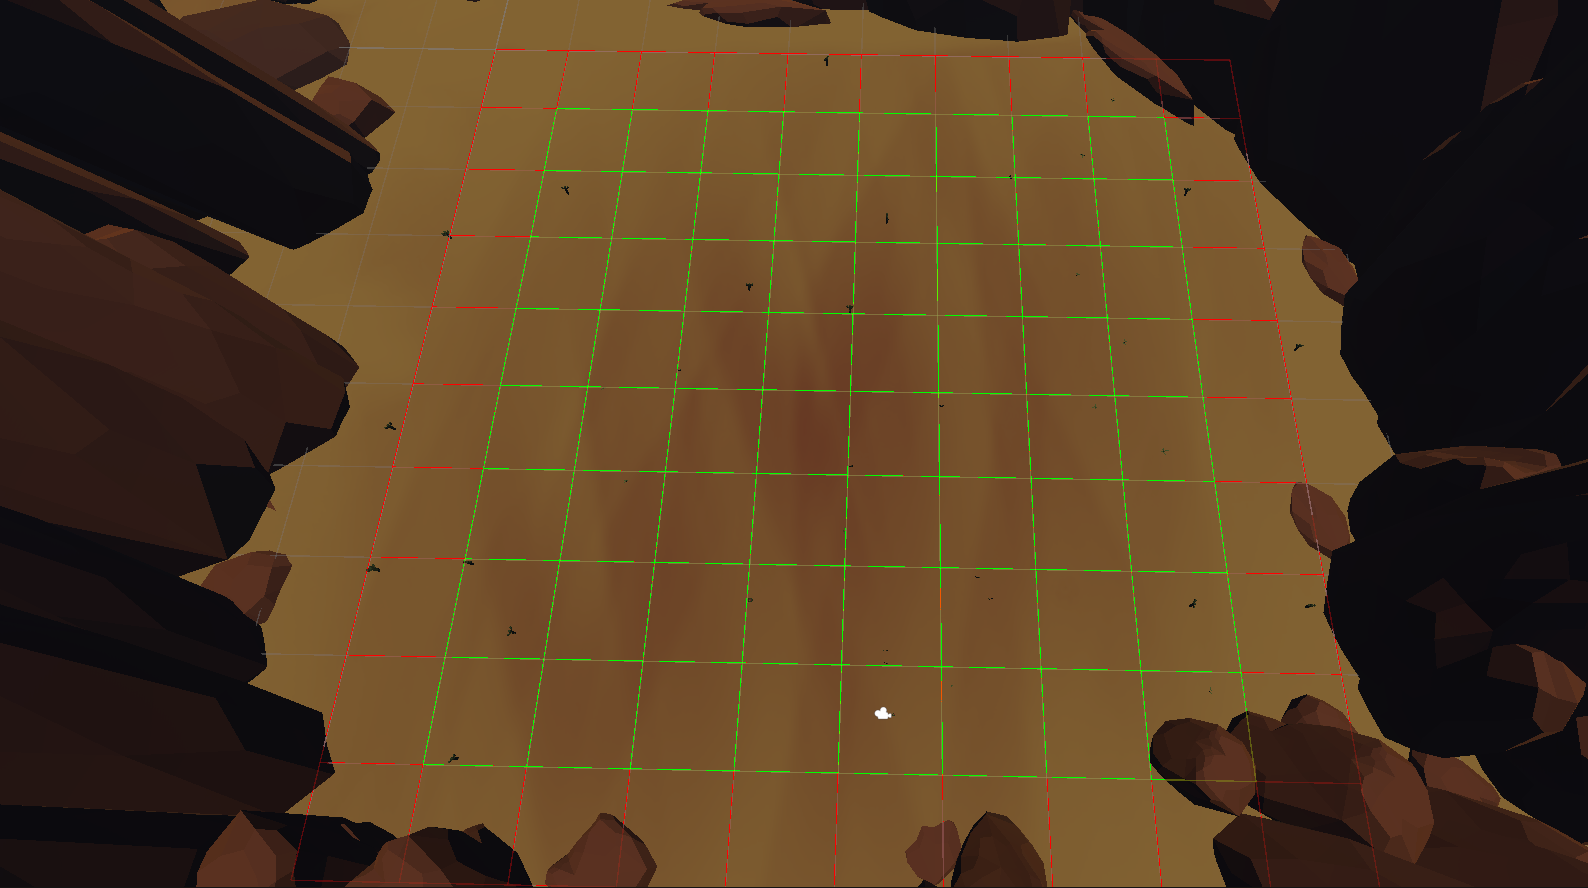
\includegraphics[width=0.5\linewidth]{map_grids.png}
    \caption{Grid Based Map}
    \label{fig:Grid-Based-Map}
\end{figure}

\section{Player Mechanics}
The player assumes the role of a commander with the ability to interact with the game world and the enemy commander.

\begin{itemize}
    \item The player can place soldiers, tanks, and throw airstrikes onto the map.
    \item The player can engage in dialogue with the enemy commander to negotiate surrender or to provoke them.
\end{itemize}

\section{Enemy Commander}
The enemy commander is powered by a large language model (LLM) and plays a pivotal role in the game.
\begin{itemize}
    \item The enemy commander interacts with the player through contextual dialogue, responding to game state changes and player actions.
    \item The NPC adjusts its "aggressiveness" and "surrender likelihood" values based on the evolving game state. (If player provokes NPC, aggressiveness increase and if the battle is going against NPC, surrender likelihood increase.)
    \item The NPC exhibits more aggressive dialogue when its aggressiveness value is high.
\end{itemize}

\section{Unit Types}
The game features three primary unit types, each with distinct roles and abilities:
\begin{itemize}
    \item \textbf{Soldiers}: Infantry units equipped with rifles that deal direct damage to targeted enemies.
    \item \textbf{Tanks}: Tank units capable of delivering area damage around a targeted enemy.
    \item \textbf{Airstrikes}: Aerial projectiles that inflict area damage at a specified location, offering strategic advantages in eliminating clusters of enemies.
\end{itemize}

\section{Victory Conditions}
The game ends when one of the following conditions is met:
\begin{itemize}
    \item \textbf{Player Victory}: Achieved by either forcing the enemy commander to surrender or eliminating all enemy units.

    \item \textbf{Enemy Victory}: The player loses if their units are obliterated.
\end{itemize}

\section{Level Design Window}
The level design window enables players to customize game settings, providing flexibility and variety for gameplay scenarios.

\subsection{Interface Overview}
The interface includes:
\begin{itemize}
    \item \textbf{Unit Configuration}: Input fields for setting player and enemy soldiers, tanks, and airstrikes.
    \item \textbf{Aggressiveness Slider}: Adjusts the enemy's behavior dynamically.
    \item \textbf{Language Button}: Toggles between English and Turkish for NPC dialogue.
    \item \textbf{Start Button}: Launches the game with the selected settings.
\end{itemize}

\subsection{Impact on Gameplay}
The level design window allows players to:
\begin{itemize}
    \item Customize difficulty by modifying unit counts and aggressiveness.
    \item Tailor gameplay scenarios to test strategies and configurations.
\end{itemize}

\subsection{Example Configuration}
A sample setup could include 30 soldiers, 10 tanks, and 5 airstrikes for the player; 40 soldiers, 8 tanks, and 7 airstrikes for the enemy; and an aggressiveness value of 3. \ref{fig:level-design-window}
\begin{figure}[!htbp]
    \centering
    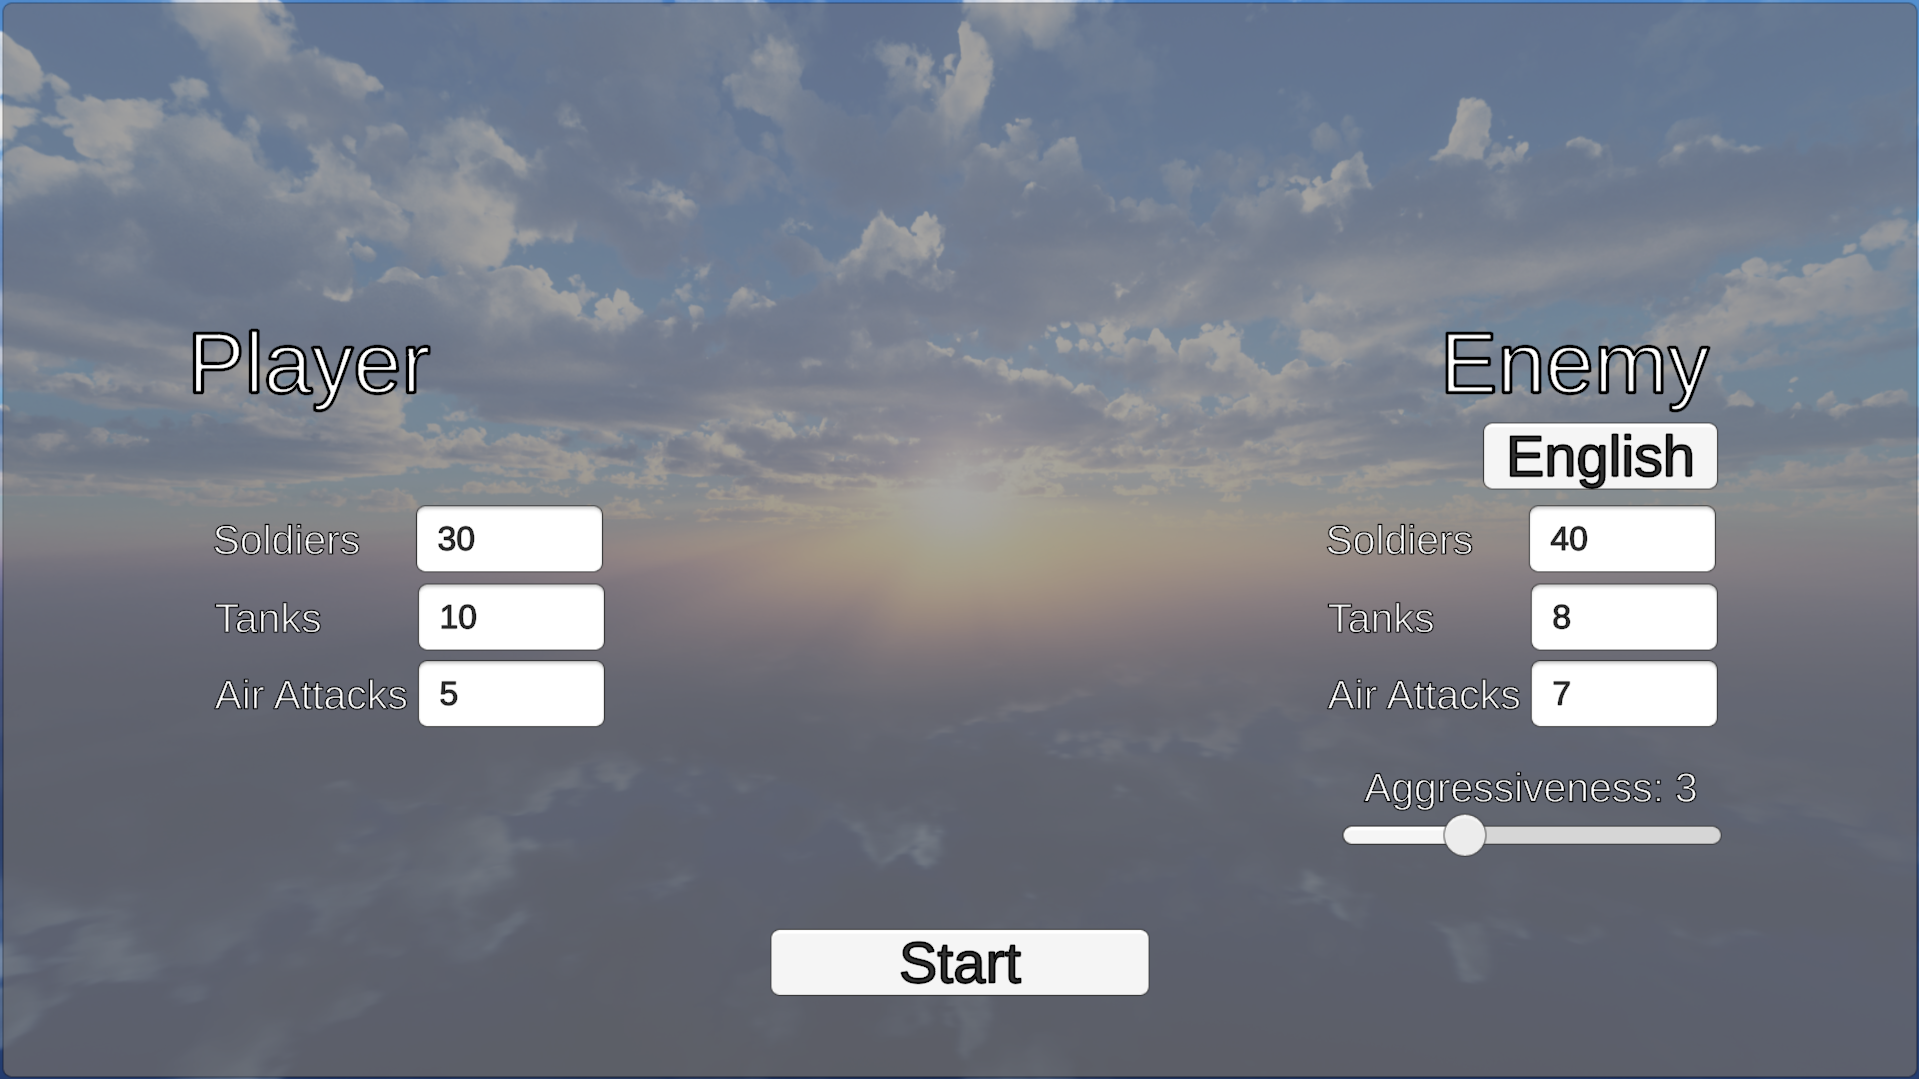
\includegraphics[width=1.0\linewidth]{image.png}
    \caption{Level Design Window}
    \label{fig:level-design-window}
\end{figure}






\chapter{Army Implementation}

The army system in the game is implemented to handle various unit types, manage their attributes, and provide dynamic behaviors during gameplay. The implementation is structured around the concepts of army information, unit attributes, and unit controllers. Each unit type is uniquely designed to fulfill specific battlefield roles, categorized as Soldiers, Tanks, and Airstrikes.

\section{Army Information}
The \texttt{Army Information} mechanism manages the overall state of the army. It tracks the following attributes:
\begin{itemize}
    \item \textbf{Initial Army}: The starting composition of soldiers, tanks, and airstrikes.
    \item \textbf{At Hand}: Units that are ready for deployment but not yet on the battlefield.
    \item \textbf{At Battlefield}: Units currently deployed and engaged in combat.
    \item \textbf{Current Total}: The combined count of units across all states, calculated dynamically.
\end{itemize}
This structure enables efficient resource tracking and provides insights into the player's and enemy's available forces during the game.

\section{Soldiers}
Soldiers are the most basic units, designed for direct combat. Their implementation involves:
\begin{itemize}
    \item \textbf{Attributes}: Managed using the \texttt{Army Member} system, soldiers have health and damage values. These attributes define their combat effectiveness.
    \item \textbf{Controller}: The \texttt{Soldier Controller} mechanism governs the behavior of soldier units, including:
    \begin{itemize}
        \item Movement towards the closest enemy.
        \item Shooting animations and effects using particle systems.
        \item Health reduction upon taking damage.
        \item Death handling, which decreases the soldier count in the battlefield and cleans up the game object.
    \end{itemize}
\end{itemize}

\section{Tanks}
Tanks are armored units with higher durability and the ability to deal area-of-effect damage. Their implementation includes:
\begin{itemize}
    \item \textbf{Attributes}: Tanks possess higher health and damage values compared to soldiers, making them suitable for breaking enemy lines.
    \item \textbf{Projectile System}: Manages the behavior of all projectiles.
    \begin{itemize}
        \item Area damage calculations based on a specified radius.
        \item Particle effects for explosions and impacts.
        \item Collision detection to determine affected units.
    \end{itemize}
    \item \textbf{Controller}: The \texttt{Tank Controller} mechanism manages tank-specific behaviors:
    \begin{itemize}
        \item Movement towards enemy targets.
        \item Turret rotation for precise aiming.
        \item Firing projectiles at enemy units.
        \item Death handling, Reduces the tank count in the battlefield and triggers visual effects, such as smoke particles, upon destruction.
    \end{itemize}
\end{itemize}

\section{Airstrikes}
Airstrikes are powerful one-time-use projectiles that target specific locations. Their implementation focuses on high-impact, strategic gameplay:
\begin{itemize}
    \item \textbf{Attributes}: Airstrikes are defined by their damage and area-of-effect radius, as they do not have health or persistent presence on the battlefield.
    \item \textbf{Behavior}: Airstrikes are deployed at a specific location and detonate on impact, dealing damage to all units within their effective radius.
    \item \textbf{Controller}: The \texttt{projectile system} is used to handle airstrike mechanics, ensuring precise targeting and explosion effects.
    \item \textbf{Particle Effects}: Explosion and impact visuals are enhanced using particle systems, providing clear feedback to the player.
\end{itemize}

\section{Army Member Controllers}
Army controllers play a vital role in managing unit behavior and interactions. Each unit type has its own controller that handles state transitions, such as:
\begin{itemize}
    \item \textbf{Idle}: Units remain stationary when no enemy is in range.
    \item \textbf{Moving}: Units navigate towards the closest enemy target.
    \item \textbf{Shooting}: Units attack the enemy when within range, applying damage.
    \item \textbf{Dead}: Units transition to a death state, triggering cleanup operations and reducing the battlefield count.
\end{itemize}

This hierarchical and modular implementation ensures that the game can manage diverse units effectively while maintaining scalable and dynamic gameplay.

\chapter{AI Implementation}

The AI system in the game is responsible for controlling the enemy commander, dynamically interacting with the player, and managing the deployment of enemy units. The implementation leverages several key components, including GPT-based interaction, attack patterns, and automated unit deployment.

\section{GPT-Driven Chat Facility}
The game's interactive dialogue system is powered by the OpenAI GPT model  \cite{openaiDotNet}. The \texttt{GPT} manages conversations with the player through the following features:
\begin{itemize}
    \item \textbf{Dynamic Dialogue}: The AI commander generates contextual responses based on the state of the game, including battlefield updates and player interactions.
    \item \textbf{Characteristics Management}: The AI adjusts its behavior, such as \texttt{anger} and \texttt{surrender likelihood}, based on the game state. These characteristics influence the tone of the AI's responses.
    \item \textbf{Secret Prompt System}: The AI is periodically updated using secret prompts (e.g., \texttt{tatata}) to integrate battlefield information and adapt its strategies accordingly.
    \item \textbf{Pre Configuration}: The AI is configured with a set of rules about the game and a sample conversation.
\end{itemize}
This system ensures the AI provides engaging and reactive dialogue, enhancing the player's experience.

\section{GPT Informer}
The \texttt{GPT Informer} is a critical component for managing and relaying information to the AI. Its primary functions include:
\begin{itemize}
    \item \textbf{Army Information Updates}: The \texttt{GPT Informer} consolidates and communicates the current state of both the enemy and player armies, including units at hand, deployed units, and overall status.
    \item \textbf{Characteristics Updates}: The AI's characteristics, such as aggressiveness and surrender likelihood, are updated dynamically using this module.
    \item \textbf{Battlefield Awareness}: By providing periodic updates, the \texttt{GPT Informer} ensures the AI remains aware of the game's current state and can make informed decisions.
\end{itemize}

\section{Attack Pattern Management}
The \texttt{Attack Pattern} structure defines the AI's unit deployment behavior based on its aggressiveness. Key features include:
\begin{itemize}
    \item \textbf{Attack Timing}: Separate attack periods are defined for soldiers, tanks, and airstrikes. These are dynamically adjusted based on the AI's aggressiveness value.
    \item \textbf{Aggressiveness Scaling}: The AI's \texttt{aggressiveness} is scaled using a divider to ensure balanced gameplay, with values clamped between 1 and 10.
    \item \textbf{Adaptive Deployment}: As the AI's aggressiveness increases, its deployment periods shorten, resulting in faster and more frequent attacks.
\end{itemize}
This system enables the AI to adapt its behavior dynamically, creating a challenging and responsive opponent.

\section{Enemy Unit Sending}
The \texttt{Enemy Unit Sending} implementation includes:
\begin{itemize}
    \item \textbf{Automated Deployment}: Separate routines are defined for deploying soldiers, tanks, and airstrikes. These routines operate on timers based on the \texttt{Attack Pattern} of the enemy.
    \item \textbf{Strategic Placement}: Units are placed at valid grid positions within the enemy territory. For airstrikes, the AI targets random positions within the player's army.
    \item \textbf{Game State Integration}: The deployment routines adapt to the current state of the game. For example, airstrikes are only deployed when the player's army exceeds a certain threshold.
    \item \textbf{Dynamic Aggressiveness}: The AI's deployment speed is influenced by its \texttt{aggressiveness}.
\end{itemize}

\section{Integration and Coordination}
The AI system integrates all components to provide a cohesive experience:
\begin{itemize}
    \item \textbf{Information Flow}: The \texttt{GPT Informer} ensures the AI has up-to-date battlefield and characteristics information.
    \item \textbf{Reactive Behavior}: The AI's dialogue and deployment strategies adapt dynamically based on inputs from the \texttt{Chat Facility} and \texttt{Enemy Unit Sending}.
    \item \textbf{Scalability}: The modular design of components like \texttt{Attack Pattern} and \texttt{Enemy Unit Sending} allows for future enhancements or adjustments to AI behavior.
\end{itemize}

This AI implementation ensures that the enemy commander is narratively engaging character with interaction and decision-making capabilities.

\chapter{Player Mechanics}

The player mechanics are designed to offer an interactive and engaging experience, allowing the player to deploy units strategically and navigate the battlefield efficiently. This chapter explains the implementation of player mechanics, focusing on unit placement, selection, and camera control.

\section{Unit Placement}
The player can deploy soldiers, tanks, and airstrikes by interacting with the battlefield. Key features include:
\begin{itemize}
    \item \textbf{Mouse Interaction}: The player clicks on valid positions on the battlefield to deploy units. A ray-cast detects if the click intersects a valid grid location.
    \item \textbf{Unit Readiness}: Before deployment, the system checks whether the selected unit type is ready and if sufficient units are available in the player's army inventory.
    \item \textbf{Deployment Logic}: The instantiation and positioning of units are handled based on the player's selection. 
\end{itemize}
This system ensures that the player's unit placement adheres to game rules and strategic limitations.

\section{Unit Selection}
The player can switch between unit types for deployment using keyboard inputs.
\begin{itemize}
    \item \textbf{Key Bindings}:
    \begin{itemize}
        \item \texttt{1}: Selects \texttt{Soldier}.
        \item \texttt{2}: Selects \texttt{Tank}.
        \item \texttt{3}: Selects \texttt{Airstrike}.
    \end{itemize}
    \item \textbf{Validation}: Selection impacts the deployment process, ensuring the player can only deploy the selected unit type if conditions are met.
\end{itemize}

\section{Camera Control}
The player has the ability to navigate and observe the battlefield. Key functionalities include:
\begin{itemize}
    \item \textbf{Movement}: The player can move the camera using the keyboard:
    \begin{itemize}
        \item \texttt{W}, \texttt{A}, \texttt{S}, \texttt{D}: Move forward, left, backward, and right, respectively.
        \item \texttt{E}: Move up.
        \item \texttt{Q}: Move down.
    \end{itemize}
    \item \textbf{Rotation}: By holding the right mouse button, the player can rotate the camera using mouse movements.
    \item \textbf{Bounds Enforcement}: The camera position is clamped within predefined bounds to prevent the player from leaving the battlefield area.
    \item \textbf{Dynamic Grid Visibility}: The system toggles the visibility of player and enemy side indicators based on camera movement.
\end{itemize}

\section{Integration with Battlefield State}
The player's mechanics are tightly integrated with the game state:
\begin{itemize}
    \item The \texttt{attack pattern} of the enemy NPC is synchronized with the player's deployment logic, maintaining balanced gameplay.
    \item The system dynamically updates the readiness status and stacks for soldiers, tanks, and airstrikes, ensuring real-time feedback on unit availability.
\end{itemize}

This comprehensive implementation allows the player to strategize effectively, engage with the battlefield dynamically, and make informed decisions during gameplay.

\chapter{Evaluation}

This project implemented a grid-based strategy war game with dynamic and interactive gameplay elements powered by an LLM. The integration of the LLM provided an enemy NPC to engage in contextual dialogue and make informed surrender decisions.

\section{Summary of Achievements}
The development of the game included several notable accomplishments:
\begin{itemize}
    \item A robust grid-based battlefield where both the player and the NPC can deploy units strategically.
    \item An LLM-powered enemy commander capable of interacting dynamically with the player and adjusting its surrender likelihood and aggressiveness based on the game state.
    \item The implementation of diverse unit types, including soldiers, tanks, and airstrikes, with distinct behaviors and battlefield roles.
    \item Seamless integration of player mechanics, allowing unit deployment, selection, and battlefield navigation.
    \item Real-time AI adjustments to game dynamics through the \texttt{Attack Pattern}, \texttt{GPT Informer}, and chat system, ensuring a responsive and adaptive opponent.
    \item The game runs at an average of 115 fps on a system equipped with an RTX 3060 GPU and a Ryzen 5 processor.
    \item The average response time for NPC interactions is approximately 2.5 seconds.
\end{itemize}

\section{Player Feedback}
To evaluate the effectiveness of the game's AI and overall player experience, 10 participants were asked to play the game and provide feedback. The average responses to key evaluation questions were as follows:
\begin{itemize}
    \item \textbf{Accuracy of NPC surrender decisions}: The NPC's ability to make accurate surrender decisions was rated at \textbf{3.8} out of 5, indicating a reasonable alignment with player expectations but with room for improvement.
    \item \textbf{Relevance of NPC responses}: The NPC's dialogue relevance was rated at \textbf{4.1} out of 5, reflecting a strong connection between its responses and the game context.
\end{itemize}
These results highlight the strengths of the AI in creating a believable and engaging opponent while also identifying areas for future enhancement.

\section{Challenges and Limitations}
The project faced several challenges and limitations:
\begin{itemize}
    \item The accuracy of surrender decisions, while reasonable, could be further refined by improving the underlying decision-making logic and incorporating additional battlefield parameters.
    \item The use of OpenAI's API introduces a dependency on an external, priced platform. This not only increases the operational cost of the project but also adds latency to response due to communication with a remote server.
\end{itemize}

\section{Future Work}
Building on the current implementation, several areas for future improvement have been identified:
\begin{itemize}
    \item Enhancing the decision-making process for NPC surrender likelihood by incorporating more sophisticated game state analysis.
    \item Expanding the diversity of unit types and their behaviors to add strategic depth.
    \item Refining the LLM's conversational logic to further improve dialogue relevance and player engagement.
    \item Conducting larger-scale play-testing to gather more comprehensive feedback and fine-tune the AI's performance.
\end{itemize}
\chapter{Conclusion}
This project demonstrates the potential of integrating advanced AI into strategy games, offering both strategic challenges and narrative depth. The implementation of a grid-based war game with an LLM-driven NPC commander provides a unique gaming experience, balancing gameplay mechanics with dynamic and engaging AI behavior. With further refinements and expansions, this system can serve as a foundation for more complex and immersive strategy games in the future.




% DON'T INPUT FILES AFTER HERE
\begin{outertitles}
\clearpage
\setlength{\emergencystretch}{1em}
\printbibliography
\addtocontents{toc}{\protect\vspace{18pt}}
\addcontentsline{toc}{chapter}{Bibliography}
%% If you don't want a CV or appendices add a % at the beginning of the relevant line
%\chapter*{CV}
\addcontentsline{toc}{chapter}{CV}

%% Edit below this line
XXX.



%% Until here
\clearpage
%\chapter*{Appendices}
\addcontentsline{toc}{chapter}{Appendices}

\section*{Appendix 1: Some publications}

No one significant, in AAA.

\section*{Appendix 2: Some explanation}

None needed mate!
\end{outertitles}
\end{document}